\section{Rezultaty i wnioski}

\subsection{Funkcjonowanie algorytmu G-średnich}

\begin{table}[!tp]
	\centering
	\caption{Liczby klas wyliczonych przez G-means}
	\label{tabResults2}
	\begin{tabular}{|c|c|c|c|}
		\hline
		Nr paczki z MIT-BIH & Matlab & Python & Julia\\ \hline		
		100 & 16 & 16 & 16\\ \hline
		101 & 14 & 16 & 16\\ \hline
		102 & 14 & 16 & 16\\ \hline
		103 & 27 & 16 & 16\\ \hline
		104 & 29 & 16 & 16\\ \hline
		105 &  1 & 20 & 20\\ \hline
		106 & 35 & 16 & 16\\ \hline
		107 & 31 & 16 & 16\\ \hline
		108 & 32 & 15 & 15\\ \hline
		109 &  1 & 21 & 21\\ \hline
		111 & 22 & 17 & 17\\ \hline
		112 & 15 & 19 & 19\\ \hline
		113 & 13 & 16 & 16\\ \hline
		114 &  1 & 15 & 15\\ \hline
		115 & 15 & 16 & 16\\ \hline
		116 &  1 & 16 & 16\\ \hline
		117 & 23 & 16 & 16\\ \hline
		119 & 33 & 16 & 16\\ \hline
		121 & 27 & 16 & 16\\ \hline
		122 & 29 & 21 & 21\\ \hline
		123 &  1 & 16 & 16\\ \hline
		124 & 30 & 15 & 15\\ \hline
		200 & 32 & 20 & 20\\ \hline
		201 & 56 & 13 & 13\\ \hline
		202 & 29 & 21 & 21\\ \hline
		203 &  1 & 26 & 26\\ \hline
		205 &  1 & 21 & 21\\ \hline
		208 & 36 & 24 & 24\\ \hline
		209 & 21 & 31 & 31\\ \hline
		210 &  1 & 20 & 20\\ \hline
		212 & 18 & 25 & 25\\ \hline
		213 & 28 & 32 & 32\\ \hline
		214 & 33 & 18 & 18\\ \hline
		215 & 18 & 32 & 32\\ \hline
		217 & 65 & 17 & 17\\ \hline
		219 & 36 & 15 & 15\\ \hline
		220 & 22 & 16 & 16\\ \hline	
		221 & 33 & 19 & 19\\ \hline
		222 &  1 & 22 & 22\\ \hline
		223 &  1 & 18 & 18\\ \hline
		230 & 15 & 20 & 20\\ \hline
		231 & 39 & 12 & 12\\ \hline
		232 & 28 & 17 & 17\\ \hline
		233 & 42 & 24 & 24\\ \hline
		234 & 27 & 29 & 29\\ \hline
	\end{tabular}
\end{table}


\subsection{Funkcjonowanie algorytmu SVM}

\begin{figure}[!htp]
	\centering
	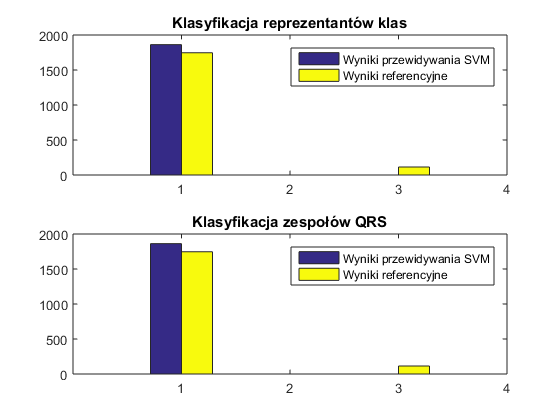
\includegraphics[width=15cm]{Grafika/101_2_3}
	\caption{Histogramy klasyfikacji zespołów dla paczki danych o numerze 101}
	\label{fig:hist1}
\end{figure}

W przypadku implementacji w Matlabie wykorzystano bibliotekę libsvm \cite{csie}. Istnieje również wersja tej biblioteki przeznaczona do wykorzystania w Pythonie, jednak po licznych, nieudanych próbach wykorzystania jej zdecydowano się zaimplementować własną maszynę wektorów nośnych w oparciu o pliki źródłowe biblioteki libsvm. Analogicznie postąpiono w przypadku implementacji w Julii. Efektem tego jest krótszy czas wykonywania się modułu napisanego w Matlabia (patrz Tab.\ref{tabResults}), a wynika między innymi z braku doświadczenia związanego z optymalizacją kodu w wykorzystanych języków programowania.

Pomiary czasu wykonywania programów napisanych w poszczególnych językach dla różnych paczek danych z bazy MIT-BIH zostały przedstawione w Tab.\ref{tabResults}.

\begin{table}[!tp]
	\centering
	\caption{Czasy wykonywania programu w poszczególnych językach dla różnych paczek danych. Wyniki wyrażone w sekundach}
	\label{tabResults}
	\begin{tabular}{|c|c|c|c|c|}
		\hline
		Nr paczki z MIT-BIH & C++ & Matlab & Python & Julia\\ \hline		
		
		100 & 2.7842 & 1.9523 & 12.8154 & 5.9019\\ \hline
		101 & 2.4618 & 1.4195 & 10.4921 & 1.8999\\ \hline
		102 & 2.7384 & 1.2609 & 12.2422 & 2.2158\\ \hline
		103 & 3.2374 & 2.3951 & 11.7082 & 2.1800\\ \hline
		104 & 2.6769 & 1.6457 & 11.8960 & 2.1335\\ \hline
		105 & 3.4991 & 1.3186 & 14.7023 & 3.1231\\ \hline
		106 & 2.3171 & 1.8217 & 10.3660 & 2.1149\\ \hline
		107 & 2.2940 & 1.5331 &  9.9881 & 2.0690\\ \hline
		108 & 1.9152 & 1.7391 &  8.5037 & 2.1076\\ \hline
		109 & 3.2367 & 1.2506 & 13.9100 & 3.4216\\ \hline
		111 & 2.6589 & 1.8369 & 11.5751 & 2.8741\\ \hline
		112 & 3.2395 & 2.2931 & 14.7076 & 3.3450\\ \hline
		113 & 2.3822 & 1.2857 & 10.2796 & 1.9384\\ \hline
		114 & 1.2847 & 0.5056 &  5.5476 & 1.5342\\ \hline
		115 & 2.7577 & 1.2325 & 11.0596 & 2.2074\\ \hline
		116 & 3.6987 & 1.242  & 13.3443 & 2.5876\\ \hline
		117 & 2.1506 & 1.506  &  8.4621 & 1.6437\\ \hline
		119 & 8.4046 & 1.5771 & 10.9920 & 2.0713\\ \hline
		121 & 2.4702 & 2.0902 & 10.2799 & 1.9764\\ \hline
		122 & 4.0723 & 2.0928 & 14.2113 & 3.1179\\ \hline
		123 & 2.0768 & 0.7942 &  8.3970 & 1.7214\\ \hline
		124 & 1.9720 & 1.6778 &  8.1376 & 1.7144\\ \hline
		200 & 2.5885 & 1.8849 & 11.5171 & 2.8278\\ \hline
		201 & 2.3562 & 1.8963 &  9.2493 & 1.8646\\ \hline
		202 & 2.7007 & 2.132  & 13.7891 & 3.7784\\ \hline
		203 & 3.1012 & 1.2565 & 14.5795 & 3.1471\\ \hline
		205 & 3.3001 & 1.3475 & 15.0669 & 3.2603\\ \hline
		208 & 4.4140 & 2.4411 & 15.5731 & 3.5292\\ \hline
		209 & 3.9942 & 2.139  & 17.3970 & 4.0028\\ \hline	
		210 & 3.2321 & 1.1721 & 26.9134 & 6.4331\\ \hline
		212 & 3.5982 & 2.9475 & 26.8902 & 3.3901\\ \hline
		213 & 4.1917 & 2.3988 & 31.4794 & 4.1461\\ \hline
		214 & 2.6582 & 1.8288 & 18.5719 & 2.4209\\ \hline
		215 & 4.5147 & 1.6584 & 30.4394 & 3.9549\\ \hline
		217 & 2.5368 & 2.0103 & 18.7012 & 2.5877\\ \hline
		219 & 2.8246 & 1.8043 & 19.7484 & 3.2817\\ \hline
		220 & 2.7018 & 1.2670 & 18.7101 & 2.6660\\ \hline		
		221 & 3.0609 & 1.7631 & 13.7086 & 3.0062\\ \hline
		222 & 3.1459 & 1.2655 & 14.3837 & 3.2238\\ \hline
		223 & 3.0877 & 1.2356 & 13.7317 & 3.0060\\ \hline
		230 & 2.7823 & 1.8286 & 14.1915 & 2.8759\\ \hline
		231 & 2.0888 & 1.4458 &  8.6989 & 3.3912\\ \hline
		232 & 2.2694 & 1.3707 & 10.3214  & 2.355\\ \hline
		233 & 3.4706 & 2.5759 & 15.5837 & 3.4776\\ \hline
		234 & 3.3963 & 3.6223 & 16.4922 & 3.5836\\ \hline
		\textbf{Czas średni} & \textbf{3.029401} & \textbf{1.5836} & \textbf{20.6123} & \textbf{2.3554}\\ \hline
	\end{tabular}
\end{table}

\subsection{Wnioski}

Krótki czas wykonywania programu napisanego w Matlabie wynika głównie z wykorzystania biblioteki libsvm, która jest napisana w C. Dla pozostałych języków zaimplementowano maszynę wektorów nośnych w oparciu o pliki źródłowe wspomnianej biblioteki.

Wykorzystanie metody SVM z szesnastoelementowym wektorem cech wydaje się złym rozwiązaniem, gdyż niemal zawsze wektor klasyfikowany jest do jednej klasy - patrz Rys.\ref{fig:hist1}. Poza zbyt licznym wektorem cech wpływ na to ma również fakt, że około 90\% zespołów QRS z bazy MIT-BIH reprezentują pobudzenia nadkomorowe. Rozwiązaniem problemu klasyfikacji może okazać się odpowiednie zmniejszenie liczności wykorzystywanego wektora cech.

Przeprowadzono również testy, w których SVM korzystał z różnych modeli (wygenerowanych z różnych paczek danych). Zaobserwowano, że normalizacja wektorów uczących znacznie przyspiesza proces uczenia, czego potwierdzeniem jest Rys.\ref{fig:SVM}.

\begin{figure}[!htp]
	\centering
	\includegraphics[width=15cm]{Grafika/SVMTrain}
	\caption{Wpływ normalizacji na czas nauki SVM}
	\label{fig:TrainNormSVM}
\end{figure}



<Coś o gmeans - że w C++ nie było, a tutaj jest>

